
\documentclass[a4paper,12pt]{article} % добавить leqno в [] для нумерации слева

\usepackage[left=2cm,right=2cm,
top=2cm,bottom=2cm,bindingoffset=0cm]{geometry}

\usepackage{amsmath,amsfonts,amssymb,amsthm,mathtools} % AMS
\usepackage{icomma} 
\mathtoolsset{showonlyrefs=true} % Показывать номера только у тех формул, на которые есть \eqref{} в тексте.
\usepackage{euscript}	 % Шрифт Евклид
\usepackage{mathrsfs} % Красивый матшрифт
\usepackage{enumitem}
\usepackage{siunitx}
\usepackage{tikz} % To generate the plot from csv
\usepackage{pgfplots}

%%% Заголовок
\author{Kseniia Kasianova}
\title{Macroeconomics. Homework 1}
\date{\today}

\newcommand{\latinword}[1]{\textsf{\itshape #1}}%

\begin{document}

{\color{blue} \latinword{Begin to write your assignment here}}

\noindent\makebox[\linewidth]{\rule{\textwidth}{0.4pt}}


\subsubsection*{Question 1} 


First of all, to answer the question why are financial intermediaries useful we need to define the term. Financial intermediaries - are such institutions that accumulate surplus resources of economic agents and provide those agents, who have a shortage of financial resources, with them in the form of various kinds of debt obligations.
For example, banks, credit unions, insurance companies, pension funds, stock exchanges, etc. are considered to be financial intermediaries.

A highly developed system of financial intermediaries can perform the role of an internal market regulator and stabilizer of the economy. The higher the level of development of the financial system, the more noticeable this role can be. If we are talking about the globalization of the financial system, financial institutions can play their economic role on a global scale.

But why exactly financial intermediaries are so important in regulating and stabilizing the economy? 
First, financial intermediaries allows to implement risk diversification through the distribution of investments in various types of financial instruments. 
Second, they allow to reduce  credit risk by verifying the solvency of the borrower. They also simplify the process of finding creditors who can provide a loan on acceptable terms, which leads to the accumulation of funds and borrowers' demand for the large amounts being satisfied. 
Third, usage of an advanced system of financial intermediaries leads to the economies of scope and scale, meaning that these institutions 
reduce the costs of information production and transaction costs of lending and borrowing. 
Fourth, financial intermediaries also facilitate such processes like maturity transformation, which is conversion of short-term liabilities (deposits) to long-term assets (loans), or asset transformation, which refers to the process of risk sharing or turning risky assets to safer ones, that also stabilizes the economy. 
 
 It all means, that creating an effective infrastructure of 
 financial intermediaries  will provide an efficient system with   fair pricing
with  low-risks, secure  system of control and proper funding.
 
\subsubsection*{Question 2  }
In the table  ''Primary Assets and Liabilities of financial intermediaries''  we see how different types of financial intermediaries raise and use   their funds. Banks (oк depositary institutions), for example, make different kinds of loans and accept deposits. Over time the distinction between subtypes of depository institutions have blurred, because their functions are quite alike, since they provide business and consumers with funds, while collecting resources in the form of deposits.  Contractual savings institutions, like insurance companies and pension funds, acquire funds on a contractual basis periodically. Since insurance companies and pension funds  usually have enough information to predict the amount of benefits they will have to pay out, liquidity of the assets is less important to them than to banks and that's why they invest in long-term securities.  Most of investment intermediaries (finance companies, mutual and hedge funds) raise funds by issuing or purchasing  stocks and bonds, they use invest their resources in financial instruments, foreign currencies and other assets.   

 Today financial intermediaries' role is becoming  more and more important. Data shows that since 1980 value of asset for each type of financial intermediaries grew increasingly   over the  years. That can be easily explained if we recollect the functions they perform, which are  reduction of transaction costs including through economy of scale,  maturity and liquidity transformation, risk sharing and diversification, reduction of asymmetry of information, etc. Each of these functions helps to facilitate the operation of financial markets and economy on the whole. 

\subsubsection*{Question 3  }
To see the difference between bonds and stocks, we need the definitions of the terms. 
Stock is a type of security, which fixes  the rights of its owner (or shareholder) to receive part of the profits of the  company which issued them  in the form of dividends, and/or participate in the management of this company, and even  receive a portion of the property  after company  goes bankrupt.
Bond is a type of a debt security, which gives its owner the right to receive from the issuer of the bond  within the agreed period of time its nominal value in cash or  another asset, and/or receive interest  from its face value (coupon), or other property rights.

These securities differ, especially  from the purchaser point of view. First, the holder of a share is a co-owner of a joint-stock company, while the holder of a bond is a creditor. Thus the shareholder has a right to vote at the general meeting of shareholders, while the owner of the bond does not, 
 though in most of the cases a shareholder has none or insignificant power in company management unless he has a large proportion of shares.

Second, stock is an irredeemable or undated asset, it exists while the joint-stock company is working, but  bond is a term security and is issued for a strictly fixed period of time. Also earnings on shares are not fixed and depend on the profit of the joint-stock company, when for bonds  a strictly established amount is paid. For a purchaser of these securities it means that the amount of money he can benefit will be calculated differently.  
 
 Thus, shares are one of the most risky and profitable investment products. Their acquisition does not guarantee a stable income, usually a purchaser benefit more from reselling a share that increased in price more than from dividends that share gives him a right for. At the same time investments in bonds are reliable and can be recommended for those who are interested in safety of capital with a low level of income.
 


\subsubsection*{Question 4  }

Starting with the definitions of these terms,  we have:

A call option is a financial agreement between two parties, a buyer, who can purchase the agreed amount of securities in the future at a price specified in the contract (strike-price) or to refuse such a purchase,   and a seller, who must sell these securities at strike-price if the buyer so decides.

A put option is a contract, that gives the buyer the right (but not the obligation) to sell a certain amount of the underlying asset to the option seller at a fixed price (strike-price). 

A European, put or call, option  gives a right to purchase or sell an asset  
at expiration date,  while a holder of an American option may
exercise the option at any time before the expiration date. The yield on an option for parties  depends on the change in the market price of the underlying asset. 

\begin{enumerate}
	\item In our case we have European options on
Ford Motor Company, with call option premium and put option premium as a function of
the strike price 
 represented on  a graph:



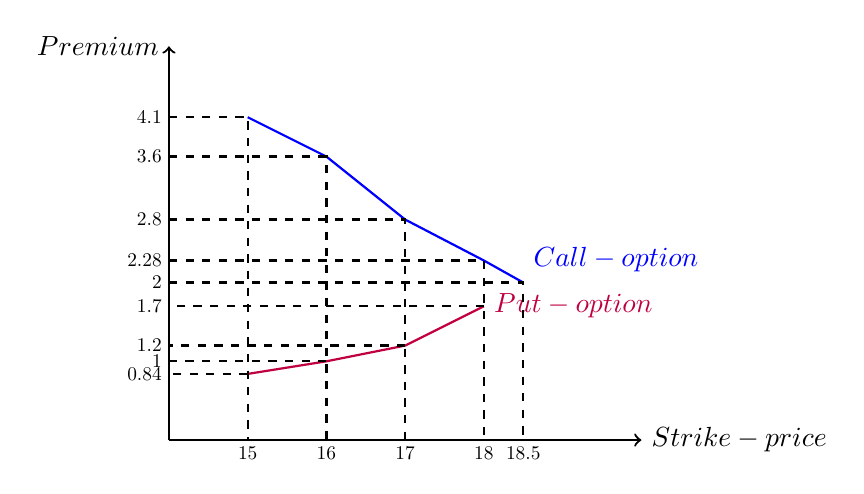
\begin{tikzpicture}[domain=0:5,scale=1,thick]
\usetikzlibrary{calc}   %allows coordinate calculations.


\draw[blue] (1, 4.1) --  (2, 3.6) -- (3, 2.8) -- (4, 2.28)  -- (4.5, 2) node[above right] {$Call-option$};



\draw[purple] (1, 0.84) --  (2, 1) -- (3, 1.2) -- (4, 1.7)    node[right] {$ Put-option  $};


% Draw axes, and dotted equilibrium lines.
\draw[->] (0,0) -- (6,0) node[right] {$Strike-price$};
\draw[->] (0,0) -- (0,5) node[left] {$Premium$};

%Price floor and ceiling lines
\draw[dashed] (0,4.1) -- (1, 4.1) -- (1,0) node[below,scale=0.7] {$15$};
\draw[dashed] (0,3.6) -- (2, 3.6) -- (2,0) node[below,scale=0.7] {$16$};
\draw[dashed] (0,2.8) -- (3, 2.8) -- (3,0) node[below,scale=0.7] {$17$};
\draw[dashed] (0, 2.28) -- (4, 2.28) -- (4,0) node[below,scale=0.7] {$18$};
\draw[dashed] (0, 2) -- (4.5, 2) -- (4.5,0) node[below,scale=0.7] {$18.5$};

\draw[dashed]  (1, 0.84) -- (0, 0.84) node[left,scale=0.7] {$0.84$};
\draw[dashed]  (2, 1) -- (0, 1) node[left,scale=0.7] {$1$};
\draw[dashed]  (3, 1.2) -- (0, 1.2)  node[left,scale=0.7] {$1.2$};
\draw[dashed]  (4, 1.7) -- (0,1.7) node[left,scale=0.7] {$1.7$};


\node [left,scale=0.7] at (0,4.1) {$ 4.1 $};
\node [left,scale=0.7] at (0,3.6) {$ 3.6 $};
\node [left,scale=0.7] at (0,2.8) {$ 2.8 $};
\node [left,scale=0.7] at (0,2.28) {$ 2.28 $};
\node [left,scale=0.7] at (0,2) {$ 2 $};

\end{tikzpicture}


\item 
Assume that an investor buys call options 18 for 2.28  premium. 

Now an investor has a right to purchase, let's say, 100 shares of Ford  in the  end  of January, 2014  at 18 USD  or to refuse to do that, depending on a market situation, while Ford  must sell these securities at 18 USD if the buyer  decides so.


That situation can be shown on a graph:



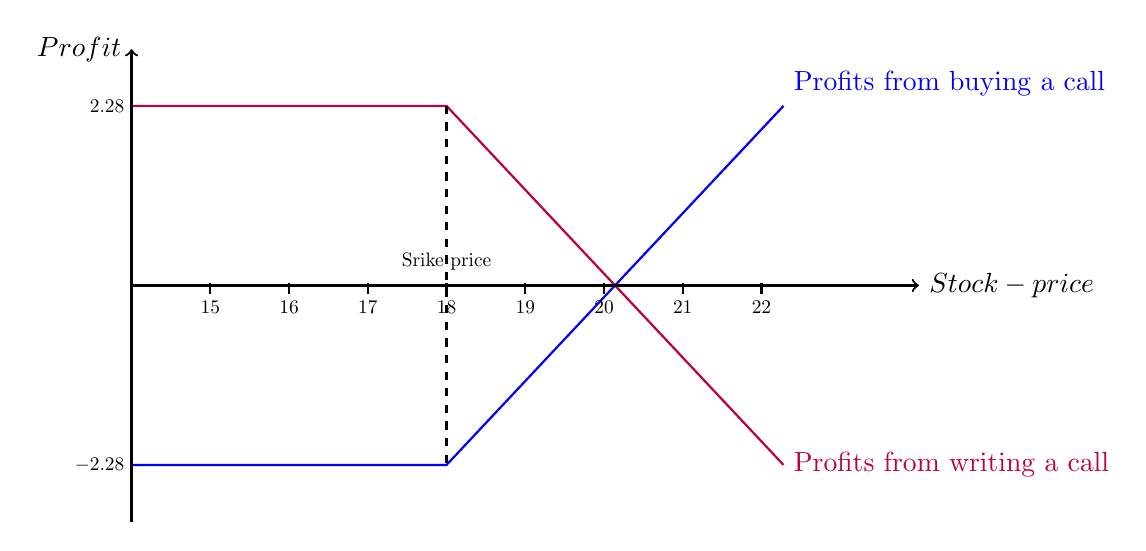
\begin{tikzpicture}[domain=0:5,scale=1,thick]
\usetikzlibrary{calc}   %allows coordinate calculations.


\draw[blue] (0, - 2.28) --  (4, -2.28)  -- (8.28,2.28) node[above right] {Profits from buying a call};

\draw[purple] (0, 2.28) -- (4, 2.28)  -- (8.28,-2.28)   node[right] {Profits from writing a call  };


% Draw axes, and dotted equilibrium lines.
\draw[->] (0,0) -- (10,0) node[right] {$Stock-price$};
\draw[->] (0,-3) -- (0,3) node[left] {$Profit$};

\foreach \x in {15,...,22} 
\draw (\x-14,1pt) -- (\x-14,-3pt) node[anchor=north,scale=0.7] {\x} ; 


%Price floor and ceiling lines
\draw[dashed] (4, 2.28) -- (4, -2.28)  ;


\node [left,scale=0.7] at (0,2.28) {$ 2.28 $};
\node [left,scale=0.7] at (0,-2.28) {$ -2.28 $};

\node [below,scale=0.7] at (4,0.5) {Srike price};

\end{tikzpicture}



The call option is beneficial for a buyer in a situation where the price of the underlying asset grows in the future,  approaching the estimated value. The financial risk is limited by the the  premium paid. 
The buyer of the call option hopes,  that the price of Ford shares  will grow higher than 18 USD by end  of January, 2014. 
When the current value of securities exceeds the estimated value, the option is executed, or "converted" into money.


\end{enumerate}

\end{document}